\documentclass[12pt,letterpaper]{article}
\usepackage[utf8]{inputenc}
\usepackage[spanish]{babel}
\usepackage{authblk}
\usepackage{graphicx} % Required for inserting images
\usepackage{charter}
\usepackage[left=1in,right=1in,top=1in,bottom=1in]{geometry}
\usepackage{verbatim}
\usepackage{hyperref}
\usepackage{natbib}

\bibliographystyle{apalike}

\setlength{\parindent}{0pt}
\setlength{\parskip}{0.6em}
\hypersetup{colorlinks=true, anchorcolor=black, urlcolor = blue, linkcolor=blue, citecolor=blue}

\title{Dise\~no experimental de la operaci\'on de monitoreo de biodiversidad}

\author{Nelson R. Salinas}
\affil{Jard\'in Bot\'anico de Bogot\'a \\ 
Grupo Conservaci\'on \emph{in situ}}
%\date{Marzo 2025}

\begin{document}

\maketitle

\section*{Introducci\'on}

El grupo de investigaci\'on ``Conservaci\'on \emph{in situ}'' del Jard\'in Bot\'anico de Bogot\'a ha incorporado entre sus objetivos para la actual vigencia el establecimiento de un programa de monitoreo de diversidad vegetal a lo largo del \'area de jurisdicci\'on del distrito. Para cumplir dicho prop\'osito es necesario implementar un dise\~no de muestreo estad\'istico.

Como variables de para orientar el dise\~no se propone utilizar la diversidad alfa de plantas vasculares (media de especies por unidad de \'area) y biomasa a\'erea vegetal (toneladas por km\textsuperscript{2}). Algunas variables accesorias pueden ser diversidad filogen\'etica, \'indices de dominancia ecol\'ogica de especies vegetales o valores de diversidad de artr\'opodos y aves.

\section*{Dise\~no}

Se propone un muestreo sistem\'atico post-estratificado de probabilidades desiguales de muestreo.
El diseño será sistemático porque los puntos de muestreo estarán distribuidos a intervalos regulares en el área de estudio.
La manera más simple de establecer sistematicidad es a través de una cuadr\'icula, cuyas celdas servir\'an como unidades principales de muestreo (\textit{psu}).
El tama\~no de estas celdas (o resoluci\'on de la cuadr\'icula) se ajustó a 4 km\textsuperscript{2}, como una manera de evitar posibles efectos de autocorrelación espacial entre muestras vecinas. 
Además, otros proyectos del grupo también han utilizado cuadrículas de la misma resolución dentro de su diseño de muestreo.
Dentro de cada celda se seleccionar\'a un solo punto de muestreo, que corresponder\'ia a la unidad secundaria de muestreo (\textit{ssu}). 

Los estratos corresponderán a clases de cobertura vegetal (páramo, bosque, etc.).
Durante esta fase exploratoria, los estratos han correspondido a la leyenda nacional de coberturas de la tierra CORINE Land Cover adaptada para Colombia \citep{ideam2010}.
Este esquema de clasificación de coberturas cuenta tanto con un producto cartográfico para el área de estudio como con un protocolo de verificación de campo, lo cual posibilita la preselección de puntos sobre coberturas asumidas y la postestratificación.

La leyenda CORINE Land Cover define bastantes coberturas en Bogotá (más de 60), demasiadas como para utilizarlas como estratos: un número alto de estratos necesariamente implica un número excesivo de unidades muestrales. Por esta razón se utilizarán nueve clases intermedias de la leyenda como estrato, de acuerdo a la agregación del cuadro \ref{tab:coberturas}.



\begin{table}
    \footnotesize
    \centering
    \begin{tabular}{|l|p{4in}|}
        \hline
        \textbf{Clase agregada} & \textbf{Leyenda} \\ \hline
        1.4. Zonas verdes artificializadas  & 1.4.1. Zonas verdes urbanas \newline 1.4.1.2. Parques cementerio \newline 1.4.1.3. Jardines botánicos \newline 1.4.2. Instalaciones recreativas \\ \hline
        %1.\{1 \& 2 \& 3\} Territorios artificializados & 1.1.1. Tejido urbano continuo \newline 1.1.2. Tejido urbano discontinuo \newline 1.2.1. Zonas industriales o comerciales \newline 1.2.1.1. Zonas industriales \newline 1.2.2. Red vial, ferroviaria y terrenos asociados \newline 1.2.2.1. Red vial y territorios asociados \newline 1.2.4. Aeropuertos \newline 1.2.5. Obras hidráulicas \newline 1.3.1. Zonas de extracción minera \newline 1.3.2. Zona de disposición de residuos\\ \hline
        2. Territorios agrícolas & 2.1.1. Otros cultivos transitorios \newline 2.1.2.1. Arroz \newline 2.1.3. Oleaginosas y leguminosas \newline 2.1.4. Hortalizas \newline 2.1.5. Tubérculos \newline 2.1.5.1. Papa \newline 2.2.1. Cultivos permanentes herbáceos \newline 2.2.1.2. Caña \newline 2.2.2.1. Otros cultivos permanentes arbustivos \newline 2.2.2.2. Café \newline 2.2.3. Cultivos permanentes arbóreos \newline 2.2.3.2. Palma de aceite \newline 2.2.3.4. Mango \newline 2.2.4. Cultivos agroforestales \newline 2.2.5. Cultivos confinados \newline 2.3.1. Pastos limpios \newline 2.3.2. Pastos arbolados \newline 2.3.3. Pastos enmalezados \newline 2.4.1. Mosaico de cultivos \newline 2.4.2. Mosaico de pastos y cultivos \newline 2.4.3. Mosaico de cultivos, pastos y espacios naturales \newline 2.4.4. Mosaico de pastos con espacios naturales \newline 2.4.5. Mosaico de cultivos con espacios naturales \\ \hline
        3.1. Bosques & 3.1.1.1.1. Bosque denso alto de tierra firme \newline 3.1.1.2.1. Bosque denso bajo de tierra firme \newline 3.1.2.1.1. Bosque abierto alto de tierra firme \newline 3.1.2.2.1. Bosque abierto bajo de tierra firme \newline 3.1.2.2.2. Bosque abierto bajo inundable \newline 3.1.3.1. Bosque fragmentado con pastos y cultivos \newline 3.1.3.2. Bosque fragmentado con vegetación secundaria \newline 3.1.4. Bosque de galería y ripario \newline 3.1.5. Plantación forestal \\ \hline
        3.2.1 Herbazales & 3.2.1.1.1.1.  Herbazal denso de tierra firme no arbolado \newline 3.2.1.1.1.2.  Herbazal denso de tierra firme arbolado \newline 3.2.1.1.1.3.  Herbazal denso de tierra firme con arbustos \newline 3.2.1.1.2.1. Herbazal denso inundable no arbolado \newline 3.2.1.2.2. Herbazal abierto rocoso \\ \hline
        3.2.\{2 \& 3\} Arbustales & 3.2.2.1. Arbustal denso \newline 3.2.2.2. Arbustal abierto \newline 3.2.3. Vegetación secundaria o en transición \newline 3.2.3.1. Vegetación secundaria alta \newline 3.2.3.2. Vegetación secundaria baja \\ \hline
        %Áreas abiertas & 3.3.1. Zonas arenosas naturales \newline 3.3.1.2. Arenales \newline 3.3.2. Afloramientos rocosos \newline 3.3.3. Tierras desnudas y degradadas \\ \hline
        %Áreas húmedas & 4.1.1. Zonas pantanosas \newline 4.1.2. Turberas \newline 4.1.3. Vegetación acuática sobre cuerpos de agua \\ \hline
        %Superficies de agua & 5.1.1. Ríos \newline 5.1.2. Lagunas, lagos y ciénagas naturales \newline 5.1.3. Canales \newline 5.1.4. Cuerpos de agua artificiales \newline 5.1.4.1. Embalses \\ \hline
    \end{tabular}
    \caption{Coberturas CORINE Land Cover agregadas consideradas en el diseño muestral.}
    \label{tab:coberturas}
\end{table}

Adicionalmente, se asignar\'an probabilidades diferenciales de selecci\'on a las unidades de muestreo, proporcionales al \'area del tipo de cobertura vegetal dentro del universo de muestreo.
De esta manera, se evitará el sobre-muestreo en coberturas comunes (p.e., páramos) y el sub-muestreo en coberturas escasas (p.e., bosques). 

Dado que no todas las unidades primarias de muestreo ser\'an visitadas, sino que ser\'an seleccionadas dadas sus probabilidades de muestreo, el efecto neto ser\'a que las unidades estar\'an dispersas aleatoriamente a lo largo y ancho del marco geoestad\'istico. Para esta clase de muestreos sistem\'aticos es posible utilizar los estimadores de varianza de un muestreo aleatorio simple o de un muestreo estratificado simple \citep{lohr2022}. % (Lohr, 2022).
Sin embargo, se propone utilizar la versión de \citet{hajek1964} de los estimadores de \citet{horvitz1952} para muestreo aleatorio. Por ejemplo, la varianza del total estimado ($\hat{T}$) es

$$ v(\hat{T}_y) = \sum_{i \in S} c_i \left( \frac{y_i}{\pi_i} - \hat{B} \right)^2 $$

donde $y_i$ es la observaci\'on de la variable $y$ en la unidad $i$, $\pi_i$ es la probabilidad de muestreo de la unidad $i$, $n$ el tamaño muestral,

$$ \hat{B} = \frac{\sum_{i \in S} \frac{c_i y_i}{\pi} }{ \sum_{i \in S} c_i} $$

y

$$ c_i = \frac{n}{n-1}(1 - \pi_i) $$

Para el caso de la media $\hat{\mu}$, la varianza est\'a determinada por 

$$ v(\hat{\mu}) = \frac{1}{N^2} v(\hat{T}_y) $$

donde $N$ es el numero total posible de muestras en la población.

\section*{Marco geoestadístico}

El universo muestral abarca todas las coberturas vegetales del \'area urbana y rural de la ciudad de Bogot\'a.
En este sentido se excluyen la áreas de infraestructura artificial y los cuerpos de agua.
%Se desestim\'o realizar muestreos dentro del casco urbano porque sus coberturas vegetales no cumplen con el supuesto de aleatoriedad necesario para aplicar los estimadores estad\'isticos a las variables principales. Es decir, dichas coberturas corresponden principalmente a parques urbanos o jardines, donde la distribución espacial de especies est\'a demarcada por un plan de cultivo. Esta realidad necesariamente implica que ni las especies ni los índices de diversidad de las mismas están dispuestas aleatoriamente en ese posible universo muestral.

En la figura \ref{fig:puntos} se ejemplifica un posible conjunto de muestras seleccionadas de acuerdo a los lineamientos estipulados anteriormente. Puede observarse que la densidad muestral es m\'as alta en las coberturas de menor representaci\'on (plantaciones forestales, bosques), mientras que en los p\'aramos y dem\'as ecosistemas de herbazal, la densidad es m\'inima. En esta simulaci\'on, el n\'umero de muestras designadas para la cobertura de bosque fue 28, 37 para los territorios agrícolas, 47 para los herbazales, 30 para los arbustales y 18 para las zonas verdes artificializadas. En esta simulación se asumió  que se establecerían 160 muestras, derivadas de ciclos de muestreo que cubren dos años, en los cuales se contarán con 2 brigadas que podrían visitar 1 localidad por semana durante periodos de 10 meses de contratación. 

\begin{figure}
    \centering
    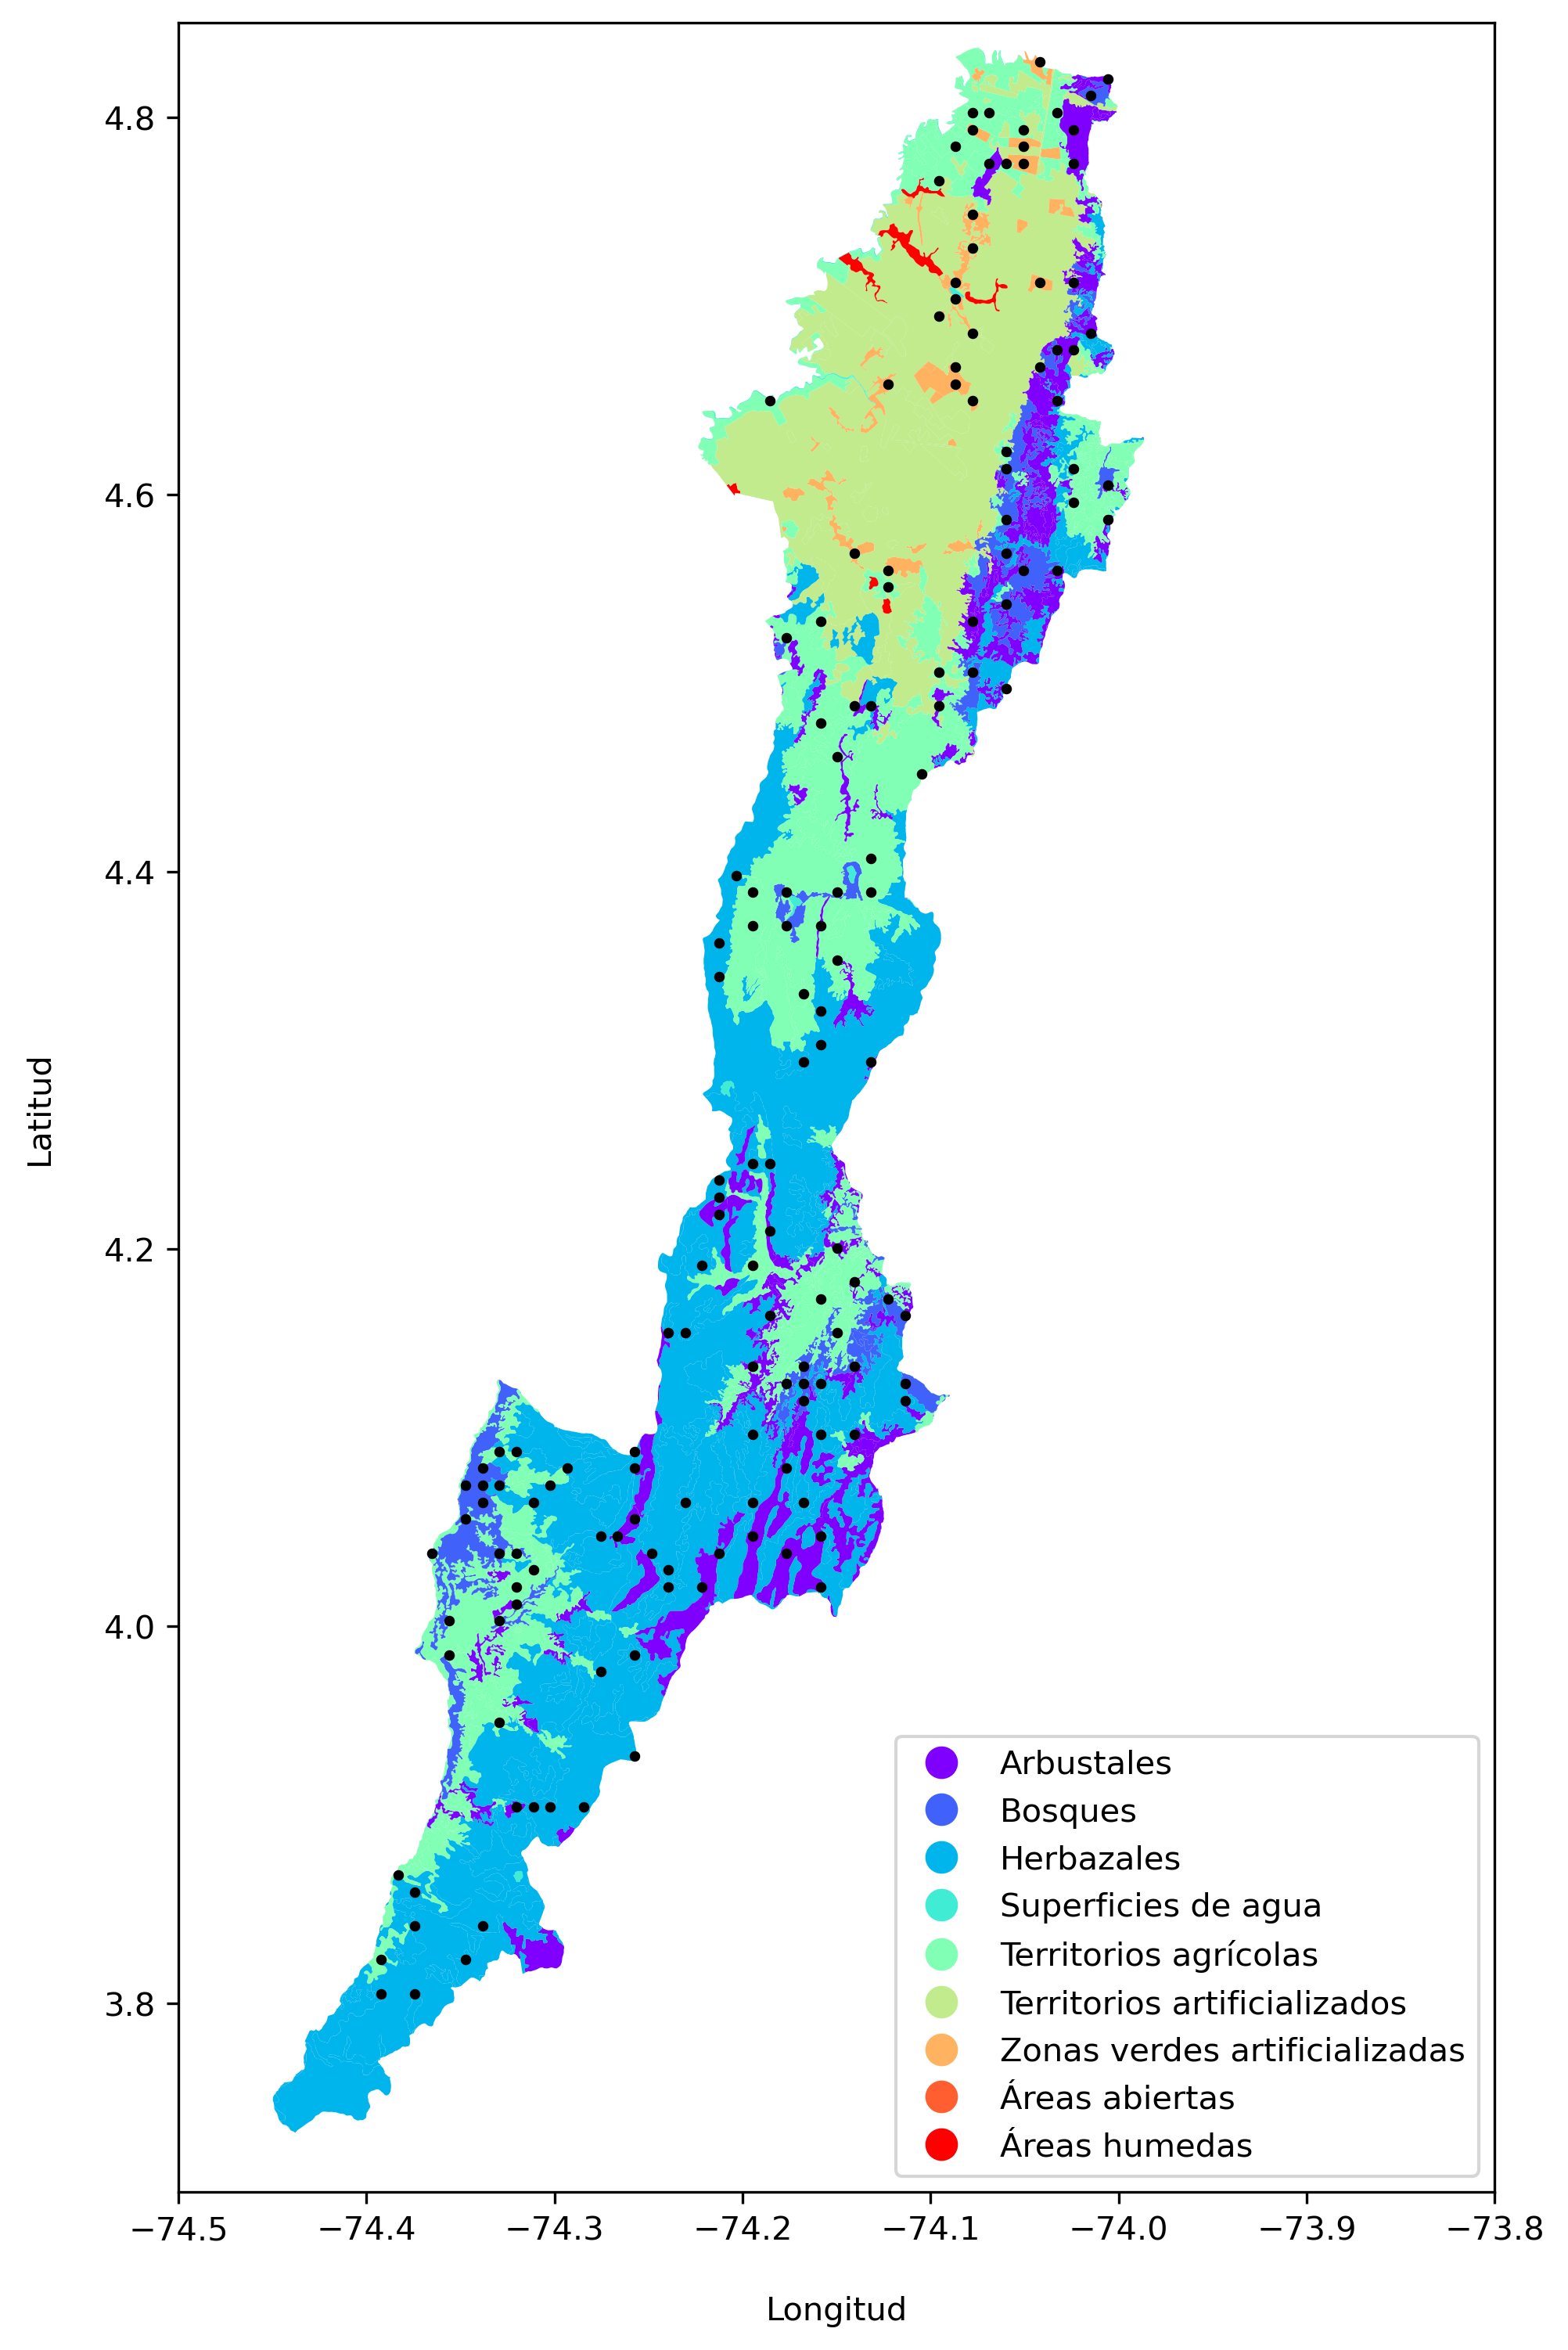
\includegraphics[height=0.9\textheight]{sitios_muestreo.png}
    \caption{Simulación de selección de puntos muestrales (n=160).}
    \label{fig:puntos}
\end{figure}


\section*{Temas pendientes por definir con el equipo}

\paragraph{Intensidad de muestreo.} Usualmente, el tama\~no muestral es definido indirectamente al seleccionar una varianza m\'axima objetivo para la variable principal. Sin embargo, en este caso no existe un conjunto de datos en el \'area de estudio que nos permita realizar una estimaci\'on preliminar de la varianza. De esta manera, la principal manera de definir el tamaño de la muestra ser\'a el costo de la operaci\'on. En las pr\'oximas semanas se realizar\'an reuniones con los dem\'as bot\'anicos del equipo para realizar una tabla de costos aproximados para cada uno de los diferentes dise\~nos de punto muestral.

\paragraph{Implementaci\'on de una estrategia de anonimizaci\'on.} En este momento no es claro si las localidades de muestreo deben ser alteradas al ser publicadas para proteger la reserva de los due\~nos de predios.


\bibliography{referencias}

\end{document}
